%%%%%%%%%%%%%%%%%%%%%
%								%
%	ESTADO DEL ARTE				%
%								%
%%%%%%%%%%%%%%%%%%%%%
\chapter{Estado del Arte}\label{cap:estadoArte}

%Por definición \textit{e-Commerce}: Transacción comercial electrónica, así como sobre Internet.
%
%Vender y realizar transacciones como estas se pueden hacer gracias a \textit{World Wide Web}, el cual es una convinación global de \textit{links}, información, paginas \textit{web} y \textit{e-Commerce websites}.
%
%Con el fin de considerar 

%TODO


\textit{Open-source \ecommerce shopping carts} ofrecen muchas ventajas para \textit{small businesses}. Soluciones \textit{Open-source} pueden ser desarrolladas para ajustarse a las necesidades del negociante. Ellos contienen una gran combinación de características a un mínimo costo. Y, aunque las opciones de soporte pueden ser mas limitadas que las propietarias o \textit{hosted platforms}, soluciones independientes \textit{open-source} generalmente tienen grandes comunidades de desarrolladores y socios para ayudar a los nuevos comerciantes.

Aquí hay una lista de 11 \textit{open-source \ecommerce solutions}. El \textit{core} de todas las aplicaciones es \textit{free}. Cada aplicación tiene extensiones \textit{free} y \textit{premium} y opciones de soporte para mejorar el desarrollo de la \textit{store}.

\newcommand{\nameOpenCart}{OpenCart }
\subsection{\nameOpenCart}

\begin{figure}[h!]
	\centering
	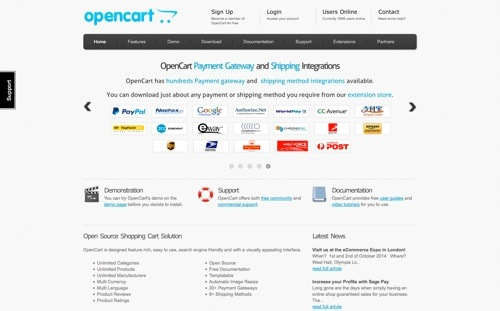
\includegraphics[width=0.5\textwidth]{figuras/cap1/openCartWebsite.jpg}
	\caption{\nameOpenCart \textit{website}\cite{online_OpenCartWebsite}.}
\end{figure}

\nameOpenCart es una aplicación \textit{open-source}, basada en PHP, es una solucion \ecommerce para comerciantes \textit{online}. \nameOpenCart tiene una comunidad activa y leal para el apoyo de usuarios, así como una lista de socios comerciales para instalación y customizacion profesional. En \nameOpenCart existen mas de 20 medios de pago, y mas de 8 métodos de envío para la descarga por defecto, con cientos de métodos adicionales para el envío y el pago en su directorio de extensiones. \nameOpenCart también fue diseñado para un manejo sencillo de múltiples compras desde una interfaz de administración. Tiene mas de 2700 \textit{themes}.

\newcommand{\namePrestaShop}{PrestaShop }
\subsection{\namePrestaShop}

\begin{figure}[h!]
	\centering
	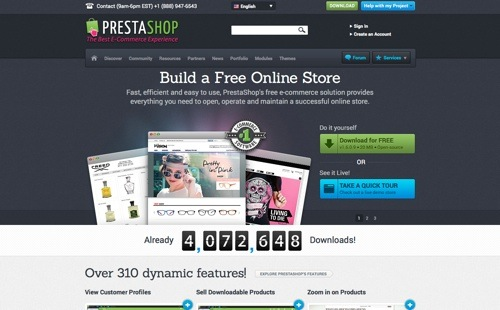
\includegraphics[width=0.5\textwidth]{figuras/cap1/PrestaShopWebsite.jpg}
	\caption{\namePrestaShop \textit{website}\cite{online_PrestaShop}.}
\end{figure}

\namePrestaShop es una solución \ecommerce \textit{open-souce}, escrita en PHP y basada en \textit{Smarty template engine}. \namePrestaShop viene con mas de 310 características integradas y 3500 modulos y \textit{templates}. Cuenta con ventas cruzadas, productos descargables, la exportación de productos, una pagina de pago, envio, descuentos y mucho mas. Descargado mas de 4 millones de veces, \namePrestaShop es usado en 160 países y traducido a 63 idiomas. Tiene mas de 600000 miembros en su comunidad.

\newcommand{\nameMagento}{Magento }
\subsection{\nameMagento Community Edition}

\begin{figure}[h!]
	\centering
	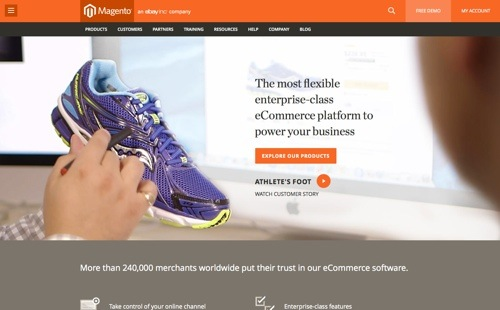
\includegraphics[width=0.5\textwidth]{figuras/cap1/MagentoWebsite.jpg}
	\caption{\nameMagento \textit{website}\cite{online_Magento}.}
\end{figure}

\nameMagento Community Edition es una version \textit{free} y \textit{open-source} de  una plataforma \ecommerce. Los comerciantes pueden acceder a caracteristicas adicionales instalando las extensiones desde el gran \textit{\nameMagento Connect marketplace}. No existe soporte para \nameMagento Community Edition, así que las respuestas a las preguntas técnicas deben ser resultas a través del foro de usuarios. Un detalle, \nameMagento ha anunciado el cierro de su \textit{hosted solution}, \nameMagento Go, por ahora no habrían problemas con Community Edition. \nameMagento Community Edition soporta mas de 200000 sitios de clientes .

\newcommand{\nameZenCart}{Zen Cart }
\subsection{\nameZenCart}

\begin{figure}[h!]
	\centering
	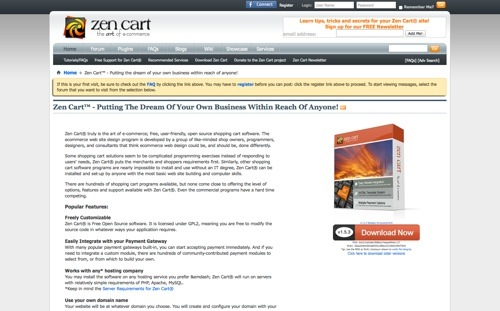
\includegraphics[width=0.5\textwidth]{figuras/cap1/ZenCartWebsite.jpg}
	\caption{\nameZenCart \textit{website}\cite{online_ZenCart}.}
\end{figure}

\nameZenCart es una aplicación \ecommerce \textit{open-source} escrita en PHP.\nameZenCart \textit{branched} desde el código osCommerce en 2003, con una solución que era mas \textit{template-based}. Tiene mas de 1800 \textit{add-ons} en 16 categorias. La comunidad de apoyo de \nameZenCart tiene aproximadamente 150000 miembros y 200000 \textit{threads}.

\newcommand{\nameSpreeCommerce}{Spree Commerce }
\subsection{\nameSpreeCommerce}

\begin{figure}[h!]
	\centering
	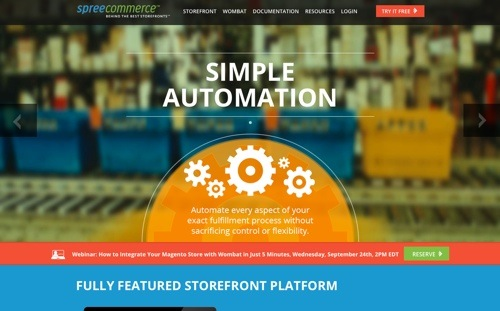
\includegraphics[width=0.5\textwidth]{figuras/cap1/SpreeCommerceWebsite.jpg}
	\caption{\nameSpreeCommerce \textit{website}\cite{online_SpreeCommerce}.}
\end{figure}

\nameSpreeCommerce es una solución \ecommerce \textit{open-source}  basado en Ruby on Rails. La plataforma modular permite configurar, complementar, o reemplazar cualquier funcionalidad que necesites. \nameSpreeCommerce tiene mas de 45000 tiendas la plataforma al rededor del mundo, incluyendo Chipotle\cite{online_Chipotle} has more than 45,000 stores using the platform around the world, including Chipotle. Spree Commerce has been translated into more than 30 languages.

\newcommand{\nameDrupalCommerce}{Drupal Commerce }
\subsection{\nameDrupalCommerce}

\begin{figure}[h!]
	\centering
	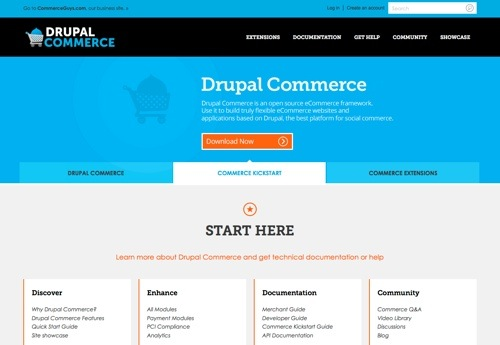
\includegraphics[width=0.5\textwidth]{figuras/cap1/DrupalCommerceWebsite.jpg}
	\caption{\nameDrupalCommerce \textit{website}\cite{online_DrupalCommerce}.}
\end{figure}	

\nameDrupalCommerce es una aplicación \ecommerce desarrollado por Commerce Guys. Construido sobre Drupal content management system. \nameDrupalCommerce ofrece un sistema de administración de producto completo, carro de compra varios lenguajes y monedas; y forma de pago. La lista de extension de \nameDrupalCommerce es una integración completamente en\textit{ third-party} para formas de pago,servicios de cumplimiento, aplicaciones de contabilidad, redes sociales y mucho mas. Paquetes de soporte técnico están disponibles por Commerce Guys.

\newcommand{\nameOsCommerce}{osCommerce }
\subsection{\nameOsCommerce}

\begin{figure}[h!]
	\centering
	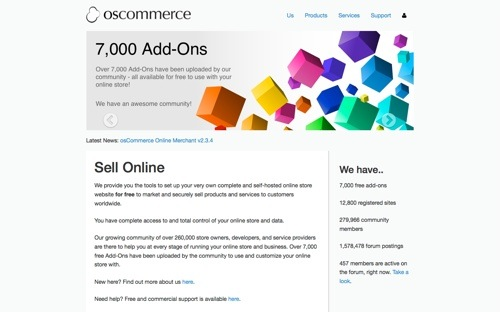
\includegraphics[width=0.5\textwidth]{figuras/cap1/osCommerceWebsite.jpg}
	\caption{\nameOsCommerce \textit{website}\cite{online_osCommerce}.}
\end{figure}

\nameOsCommerce (i.e., \textit{open source Commerce})es uno de las primeras aplicaciones \ecommerce \textit{open-source}. Mas de 7000 \textit{free add-ons} han sido subidos por su comunidad para customizar una  \textit{online store}. \nameOsCommerce es usado por cerca de 13000 sitios registrados. La comunidad de apoyo tiene aproximadamente 280000 miembros los cuales han contribuido con 1.5 millones de posts en los foros. La comunidad directa juntos con miembros de otra comunidad están disponibles en vivo en el \textit{Chat room}.

\newcommand{\nameSimpleCart}{simpleCart }
\subsection{\nameSimpleCart}

\begin{figure}[h!]
	\centering
	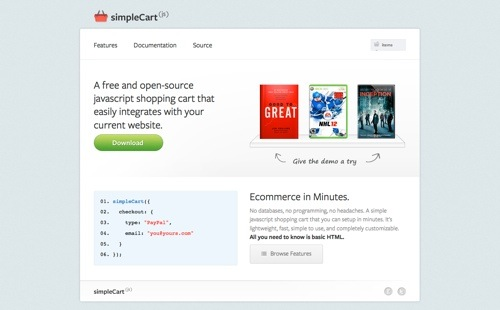
\includegraphics[width=0.5\textwidth]{figuras/cap1/simpleCartWebsite.jpg}
	\caption{\nameSimpleCart \textit{website}\cite{online_simpleCart}.}
\end{figure}

\nameSimpleCart(js) es un \textit{free} y \textit{open-source} JavaScript \textit{shopping cart}. Con su pequeño tamaño, \nameSimpleCart(js) esta disseñado para mantener simple  y sitions con alto trafico \textit{running fast}. \nameSimpleCart(js) tienen la habilidad de pagar con PayPal Express, Google Checkout, y Amazon Payments. \textit{Email checkout} e integracion con  Authorize.Net llegaran pronto.

\newcommand{\nameWooCommerce}{WooCommerce }
\subsection{\nameWooCommerce}

\begin{figure}[h!]
	\centering
	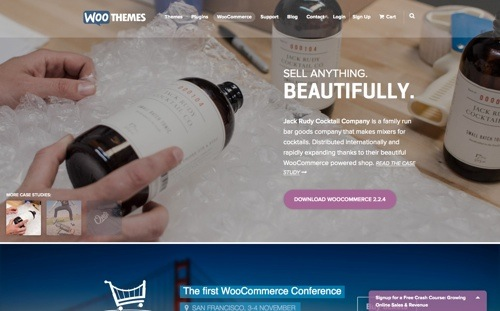
\includegraphics[width=0.5\textwidth]{figuras/cap1/WooCommerceWebsite.jpg}
	\caption{\nameWooCommerce \textit{website}\cite{online_WooCommerce}.}
\end{figure}

\nameWooCommerce es una aplicación \ecommerce \textit{free open-source} que permite a los comerciantes transformar \textit{WordPress sites} en \textit{stores}. \nameWooCommerce fue desarrollado por WooThemes desde un \textit{fork} de Jigoshop. \nameWooCommerce tiene una larga variedad de  \textit{plugins} y  \textit{themes} de WooThemes, como de sitios \textit{third party} tales como ThemeForest\cite{online_ThemeForest} y CodeCanyon\cite{online_CodeCanyon}. Con cerca de 4.5 millones de descargas desde \textit{WordPress.org}\cite{online_WordPress}, \nameWooCommerce es una solución \ecommerce muy popular para WordPress. Para obtener el soporte oficial de WooThemes, es necesario comprar un producto. De otra manera, obtener ayuda desde la comunidad activa del foro.

\newcommand{\nameWPECommerce}{WP \ecommerce }
\subsection{\nameWPECommerce}

\begin{figure}[h!]
	\centering
	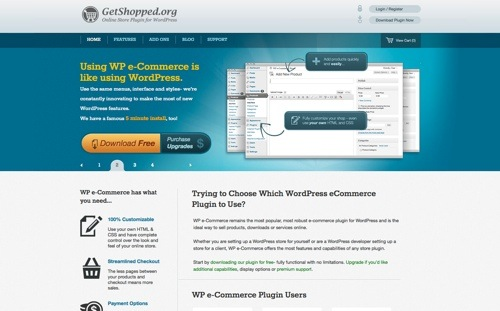
\includegraphics[width=0.5\textwidth]{figuras/cap1/WPECommerceWebsite.jpg}
	\caption{\nameWPECommerce \textit{website}\cite{online_WPECommerce}.}
\end{figure}

\nameWPECommerce es otra aplicacion popular obtenida desde la conversión del  sitio WordPress a una \ecommerce \textit{store}.\nameWPECommerce tiene cerca de 3 millones de descarga de \textit{plugin} desde \textit{WordPress.org}. Usa el propuo HTML y CSS y obten el control completo sobre la vista y la experiencia de tu \textit{online store}.\nameWPECommerce tiene una gran variedad de caracteristicas estandar, incluyendo \textit{ multi-tier pricing} para descuentos por cantidad e integración con redes sociales para \textit{marketing}. Para soporte, hay tutoriales en video y un foro en  \textit{ WordPress.org} ,tambien como consultantes de caracteristicas para ayuda profesional.

\newcommand{\nameJigoshop}{Jigoshop }
\subsection{\nameJigoshop}

\begin{figure}[h!]
	\centering
	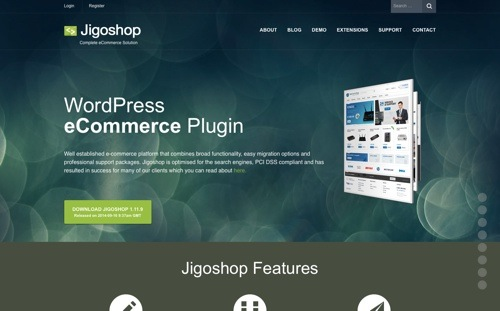
\includegraphics[width=0.5\textwidth]{figuras/cap1/JigoshopWebsite.jpg}
	\caption{\nameJigoshop \textit{website}\cite{online_Jigoshop}.}
\end{figure}

\nameJigoshop es una solución \ecommerce \textit{free} y \textit{open-source} basado en WordPress. Liberado en 2011, \nameJigoshop es el predecesor para WooCommerce. \nameJigoshop tiene mas de 30   \textit{themes}, 100 extensiones, y tres \textit{theme frameworks}. \nameJigoshop es  \textit{free}, asi como el soporte a \textit{WordPress.org}. Sin embago, el acceso a la comunidad de \textit{Jigoshop.com} comienza desde \$40 por mes.


\begin{table}[h!]
    \tiny
   
%\begin{tabular}{ |C{0.3\paperwidth}|C{0.3\paperwidth}| }
\begin{tabular}{ |l|c|c|c|c|c| }

\hline
	&
	\textit{Free database backend support}&
	Language&
	\textit{\gloss{waf}}&
	License&

\\ \hline
	\nameOpenCart &
	MySQL&
	PHP&
	&
	GPLv3&
	
\\ \hline
	\namePrestaShop &
	MySQL&
	PHP&
	&
	Open Software License&
	
\\ \hline
	\nameMagento &
	MySQL&
	PHP&
	Zend Framework\cite{online_zend_framework}&
	Open Software License&
	
\\ \hline
	\nameZenCart &
	&
	&
	&
	&
 
\\ \hline
	\nameSpreeCommerce &
	MySQL, PostgreSQL, SQLite3&
	Ruby\cite{online_ruby_language}&
	Ruby on Rails\cite{online_ruby_rails}&
	New BSD License&

\\ \hline
	\nameDrupalCommerce &
	MySQL, PostgreSQL, SQLite3&
	PHP&
	Drupal\cite{online_drupal}&
	GNU GPL&
	
\\ \hline
	\nameOsCommerce &
	&
	&
	&
	&

\\ \hline
	\nameSimpleCart &
	&
	&
	&
	&
	
\\ \hline
	\nameWooCommerce &
	MySQL&
	PHP&
	WordPress\cite{online_wordpress}&
	GNU GPL&
	
\\ \hline
	\nameWPECommerce &
	&
	&
	&
	&
	
\\ \hline
	\nameJigoshop &
	MySQL&
	PHP&
	WordPress\cite{online_wordpress}&
	GNU GPL&
	
\\ \hline
\end{tabular}
    \caption{ Comparación entre diferentes opciones \ecommerce}
    \label{tab:wide_table}
\end{table}

\begin{table}[h!]
    \tiny
   
%\begin{tabular}{ |C{0.3\paperwidth}|C{0.3\paperwidth}| }
\begin{tabular}{ |l|c|c|c|c| }
\hline
	&
	traider\cite{online_Traider}&
	ReactionCommerce\cite{online_reactionCommerce}&
	NodeShop\cite{online_NodeShop}&
	Forward\cite{online_Forward}
 
\\ \hline
	Tecnología &
	bootstrap, nodejs and mongodb &
	Nodejs, Meteor, Mongodb, CoffeScript, Bootstrap, Docker&
	&
	

\\ \hline
	Mobile &
	&
	&
	&
\\ \hline
	version &
	&
	&
	0.06 ( 21/08/2013 )&
	0.1

\\ \hline
\end{tabular}
    \caption{ Resumen tecnologías entre diferentes opciones \textit{e-Commerce}}
    \label{tab:resume_technology_ecommerce}
\end{table}

Como se observa, existe una gran cantidad de aplicaciones \textit{open-souce} las cuales están disponibles para ingresar al mundo del comercio electrónico. Todas estas opciones tienen grandes comunidades que las respaldan, así como muchos usuarios satisfechos. 

Considerando esto, ¿ habrá alguna razón que justifique el desarrollo de un proyecto de estas características?

\section{Tecnologías }\label{cap:estadoArte:tecnologias}

	\subsection{MongoDB}
	MongoDB (from "humongous") is an open-source document database, and the leading NoSQL database. Written in C++ \cite{technology_mongodb}.
	
	\subsection{Angularjs}
	\cite{technology_angularjs}
	
	\subsection{Bootstrap}
	Bootstrap is the most popular HTML, CSS, and JS framework for developing responsive, mobile first projects on the web \cite{technology_bootstrap}.
	
	\subsection{Nodejs}
	Node.js® is a platform built on Chrome's JavaScript runtime for easily building fast, scalable network applications. Node.js uses an event-driven, non-blocking I/O model that makes it lightweight and efficient, perfect for data-intensive real-time applications that run across distributed devices \cite{technology_nodejs}.
	
	\subsection{CoffeeScript}
	CoffeeScript is a little language that compiles into JavaScript. Underneath that awkward Java-esque patina, JavaScript has always had a gorgeous heart. CoffeeScript is an attempt to expose the good parts of JavaScript in a simple way.
	
	The golden rule of CoffeeScript is: "It's just JavaScript". The code compiles one-to-one into the equivalent JS, and there is no interpretation at runtime. You can use any existing JavaScript library seamlessly from CoffeeScript (and vice-versa). The compiled output is readable and pretty-printed, will work in every JavaScript runtime, and tends to run as fast or faster than the equivalent handwritten JavaScript \cite{technology_coffeescript}.
	
	\subsection{Grunt} 
	\cite{technology_gruntjs}
	
	\subsection{Docker}
	Docker is an open platform for developers and sysadmins to build, ship, and run distributed applications. Consisting of Docker Engine, a portable, lightweight runtime and packaging tool, and Docker Hub, a cloud service for sharing applications and automating workflows, Docker enables apps to be quickly assembled from components and eliminates the friction between development, QA, and production environments. As a result, IT can ship faster and run the same app, unchanged, on laptops, data center VMs, and any cloud\cite{technology_docker}.
	
	




\begin{table}[h!]
    \tiny
   
%\begin{tabular}{ |C{0.3\paperwidth}|C{0.3\paperwidth}| }
\begin{tabular}{ |L{0.1\paperwidth}|L{0.3\paperwidth}|L{0.3\paperwidth}|}
\hline
	\ecommerce&
	SQL Databases &
	NoSQL Databases
 
\\ \hline
	El \textit{schema} de los productos varia&
	\textit{Schema} rigido&
	\textit{Schema} flexible
\\ \hline
	Necesita escalar&
	&
	
\\ \hline
	Transacciones&
	&
	
\\ \hline
\end{tabular}
    \caption{ \nosql vs. \sql en relación a \ecommerce}
    \label{tab:SQL_vs_noSQL_summary}
\end{table}

	\subsection{ \textit{Full-Stack} JavaScript }
	
	%Before digging into Node.js, you might want to read up on the benefits of using JavaScript across the stack which unifies the language and data format (JSON), allowing you to optimally reuse developer resources. As this is more a benefit of JavaScript than Node.js specifically, we won’t discuss it much here. But it’s a key advantage to incorporating Node in your stack.



Recapitulando, he demostrado que las soluciones actuales de \ecommerce pueden ser considerablemente mejoradas utilizando la tecnología actualmente presente. 
Importante notar que solo estoy ofreciendo una mejor solucuón a lo que ya existe, en ningun caso indico la solución que presento es la mejor posible. No se ha realizado un estudio sobre todas las opciones disponibles del mercado. Sin embargo esta solución ofrece

speed
scalability
flexibility
performance
